\documentclass[1p]{elsarticle_modified}
%\bibliographystyle{elsarticle-num}

%\usepackage[colorlinks]{hyperref}
%\usepackage{abbrmath_seonhwa} %\Abb, \Ascr, \Acal ,\Abf, \Afrak
\usepackage{amsfonts}
\usepackage{amssymb}
\usepackage{amsmath}
\usepackage{amsthm}
\usepackage{scalefnt}
\usepackage{amsbsy}
\usepackage{kotex}
\usepackage{caption}
\usepackage{subfig}
\usepackage{color}
\usepackage{graphicx}
\usepackage{xcolor} %% white, black, red, green, blue, cyan, magenta, yellow
\usepackage{float}
\usepackage{setspace}
\usepackage{hyperref}

\usepackage{tikz}
\usetikzlibrary{arrows}

\usepackage{multirow}
\usepackage{array} % fixed length table
\usepackage{hhline}

%%%%%%%%%%%%%%%%%%%%%
\makeatletter
\renewcommand*\env@matrix[1][\arraystretch]{%
	\edef\arraystretch{#1}%
	\hskip -\arraycolsep
	\let\@ifnextchar\new@ifnextchar
	\array{*\c@MaxMatrixCols c}}
\makeatother %https://tex.stackexchange.com/questions/14071/how-can-i-increase-the-line-spacing-in-a-matrix
%%%%%%%%%%%%%%%

\usepackage[normalem]{ulem}

\newcommand{\msout}[1]{\ifmmode\text{\sout{\ensuremath{#1}}}\else\sout{#1}\fi}
%SOURCE: \msout is \stkout macro in https://tex.stackexchange.com/questions/20609/strikeout-in-math-mode

\newcommand{\cancel}[1]{
	\ifmmode
	{\color{red}\msout{#1}}
	\else
	{\color{red}\sout{#1}}
	\fi
}

\newcommand{\add}[1]{
	{\color{blue}\uwave{#1}}
}

\newcommand{\replace}[2]{
	\ifmmode
	{\color{red}\msout{#1}}{\color{blue}\uwave{#2}}
	\else
	{\color{red}\sout{#1}}{\color{blue}\uwave{#2}}
	\fi
}

\newcommand{\Sol}{\mathcal{S}} %segment
\newcommand{\D}{D} %diagram
\newcommand{\A}{\mathcal{A}} %arc


%%%%%%%%%%%%%%%%%%%%%%%%%%%%%5 test

\def\sl{\operatorname{\textup{SL}}(2,\Cbb)}
\def\psl{\operatorname{\textup{PSL}}(2,\Cbb)}
\def\quan{\mkern 1mu \triangleright \mkern 1mu}

\theoremstyle{definition}
\newtheorem{thm}{Theorem}[section]
\newtheorem{prop}[thm]{Proposition}
\newtheorem{lem}[thm]{Lemma}
\newtheorem{ques}[thm]{Question}
\newtheorem{cor}[thm]{Corollary}
\newtheorem{defn}[thm]{Definition}
\newtheorem{exam}[thm]{Example}
\newtheorem{rmk}[thm]{Remark}
\newtheorem{alg}[thm]{Algorithm}

\newcommand{\I}{\sqrt{-1}}
\begin{document}

%\begin{frontmatter}
%
%\title{Boundary parabolic representations of knots up to 8 crossings}
%
%%% Group authors per affiliation:
%\author{Yunhi Cho} 
%\address{Department of Mathematics, University of Seoul, Seoul, Korea}
%\ead{yhcho@uos.ac.kr}
%
%
%\author{Seonhwa Kim} %\fnref{s_kim}}
%\address{Center for Geometry and Physics, Institute for Basic Science, Pohang, 37673, Korea}
%\ead{ryeona17@ibs.re.kr}
%
%\author{Hyuk Kim}
%\address{Department of Mathematical Sciences, Seoul National University, Seoul 08826, Korea}
%\ead{hyukkim@snu.ac.kr}
%
%\author{Seokbeom Yoon}
%\address{Department of Mathematical Sciences, Seoul National University, Seoul, 08826,  Korea}
%\ead{sbyoon15@snu.ac.kr}
%
%\begin{abstract}
%We find all boundary parabolic representation of knots up to 8 crossings.
%
%\end{abstract}
%\begin{keyword}
%    \MSC[2010] 57M25 
%\end{keyword}
%
%\end{frontmatter}

%\linenumbers
%\tableofcontents
%
\newcommand\colored[1]{\textcolor{white}{\rule[-0.35ex]{0.8em}{1.4ex}}\kern-0.8em\color{red} #1}%
%\newcommand\colored[1]{\textcolor{white}{ #1}\kern-2.17ex	\textcolor{white}{ #1}\kern-1.81ex	\textcolor{white}{ #1}\kern-2.15ex\color{red}#1	}

{\Large $\underline{12a_{0146}~(K12a_{0146})}$}

\setlength{\tabcolsep}{10pt}
\renewcommand{\arraystretch}{1.6}
\vspace{1cm}\begin{tabular}{m{100pt}>{\centering\arraybackslash}m{274pt}}
\multirow{5}{120pt}{
	\centering
	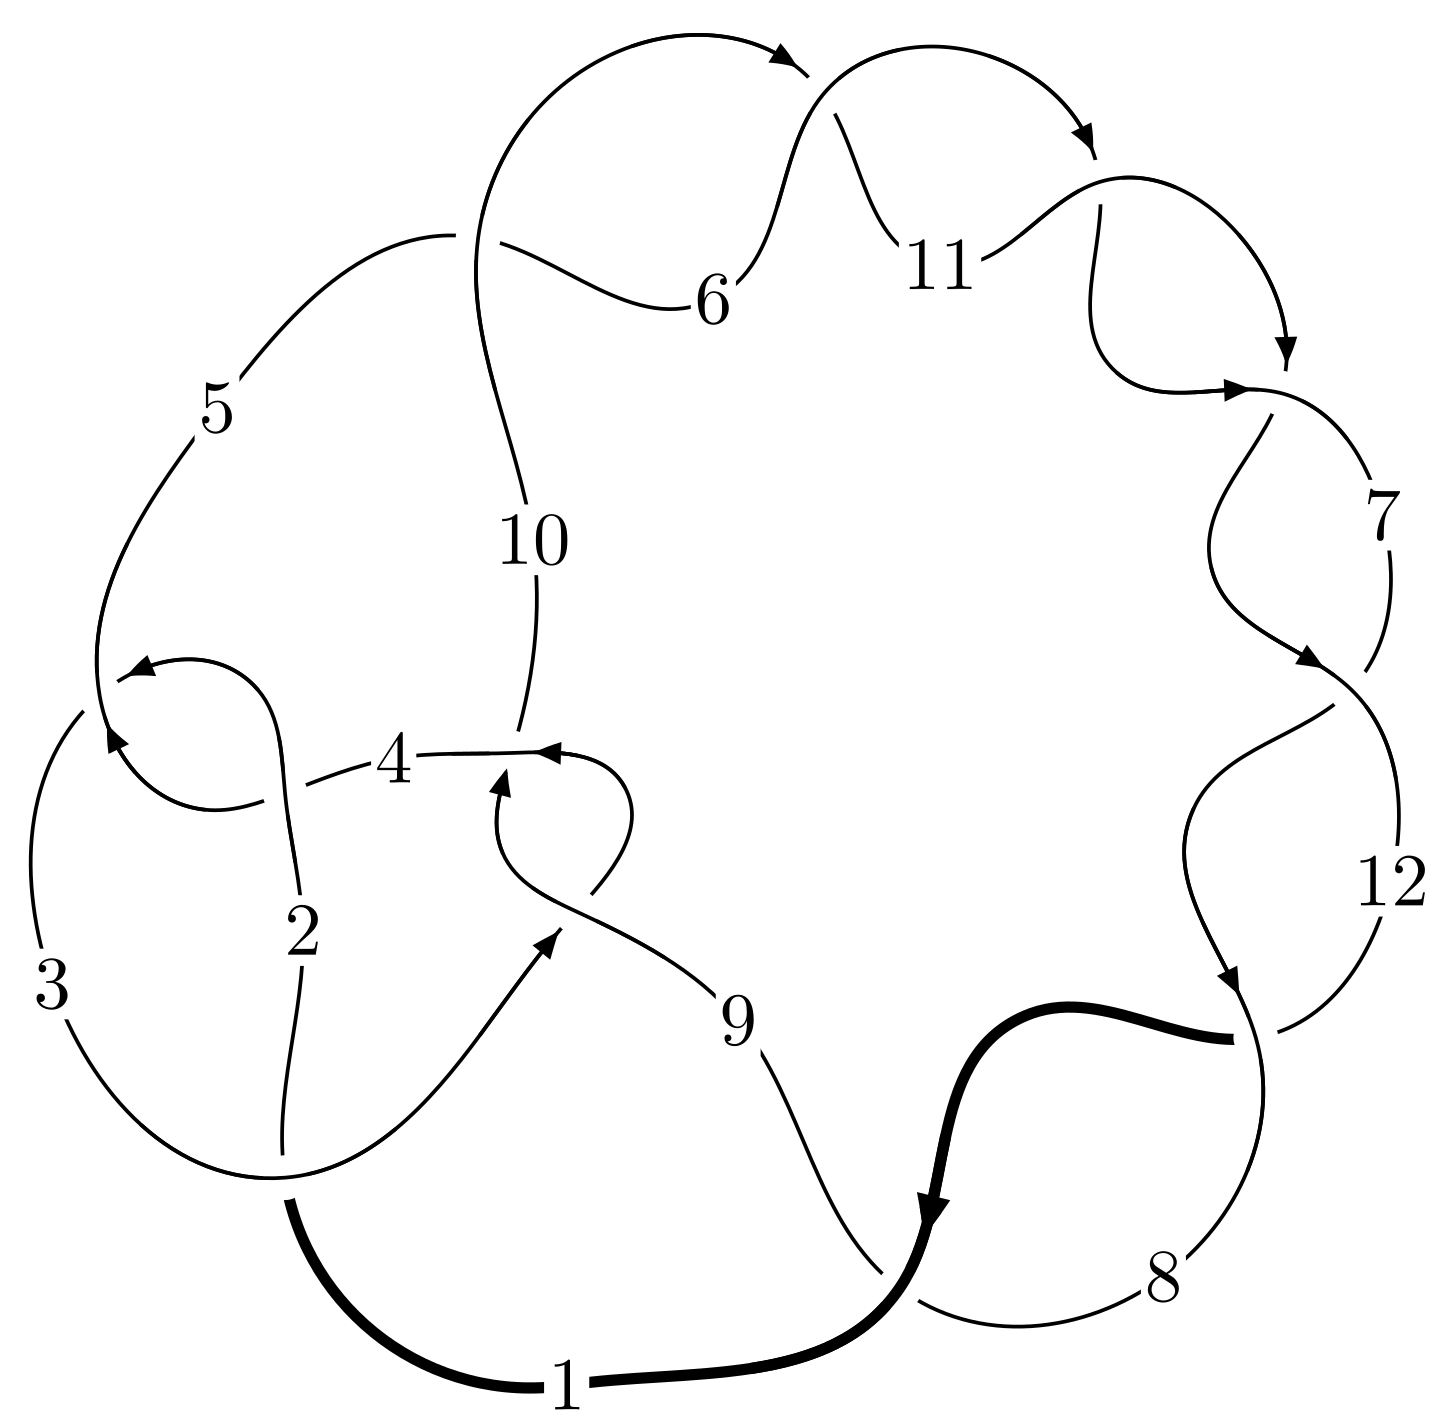
\includegraphics[width=112pt]{../../../GIT/diagram.site/Diagrams/png/947_12a_0146.png}\\
\ \ \ A knot diagram\footnotemark}&
\allowdisplaybreaks
\textbf{Linearized knot diagam} \\
\cline{2-2}
 &
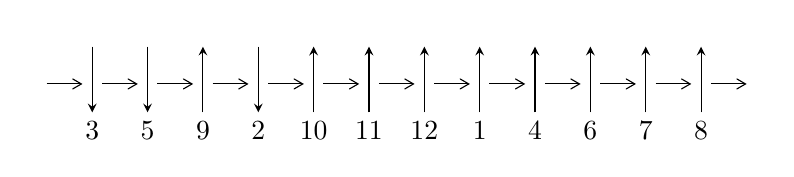
\begin{tikzpicture}[x=20pt, y=17pt]
	% nodes
	\node (C0) at (0, 0) {};
	\node (C1) at (1, 0) {};
	\node (C1U) at (1, +1) {};
	\node (C1D) at (1, -1) {3};

	\node (C2) at (2, 0) {};
	\node (C2U) at (2, +1) {};
	\node (C2D) at (2, -1) {5};

	\node (C3) at (3, 0) {};
	\node (C3U) at (3, +1) {};
	\node (C3D) at (3, -1) {9};

	\node (C4) at (4, 0) {};
	\node (C4U) at (4, +1) {};
	\node (C4D) at (4, -1) {2};

	\node (C5) at (5, 0) {};
	\node (C5U) at (5, +1) {};
	\node (C5D) at (5, -1) {10};

	\node (C6) at (6, 0) {};
	\node (C6U) at (6, +1) {};
	\node (C6D) at (6, -1) {11};

	\node (C7) at (7, 0) {};
	\node (C7U) at (7, +1) {};
	\node (C7D) at (7, -1) {12};

	\node (C8) at (8, 0) {};
	\node (C8U) at (8, +1) {};
	\node (C8D) at (8, -1) {1};

	\node (C9) at (9, 0) {};
	\node (C9U) at (9, +1) {};
	\node (C9D) at (9, -1) {4};

	\node (C10) at (10, 0) {};
	\node (C10U) at (10, +1) {};
	\node (C10D) at (10, -1) {6};

	\node (C11) at (11, 0) {};
	\node (C11U) at (11, +1) {};
	\node (C11D) at (11, -1) {7};

	\node (C12) at (12, 0) {};
	\node (C12U) at (12, +1) {};
	\node (C12D) at (12, -1) {8};
	\node (C13) at (13, 0) {};

	% arrows
	\draw[->,>={angle 60}]
	(C0) edge (C1) (C1) edge (C2) (C2) edge (C3) (C3) edge (C4) (C4) edge (C5) (C5) edge (C6) (C6) edge (C7) (C7) edge (C8) (C8) edge (C9) (C9) edge (C10) (C10) edge (C11) (C11) edge (C12) (C12) edge (C13) ;	\draw[->,>=stealth]
	(C1U) edge (C1D) (C2U) edge (C2D) (C3D) edge (C3U) (C4U) edge (C4D) (C5D) edge (C5U) (C6D) edge (C6U) (C7D) edge (C7U) (C8D) edge (C8U) (C9D) edge (C9U) (C10D) edge (C10U) (C11D) edge (C11U) (C12D) edge (C12U) ;
	\end{tikzpicture} \\
\hhline{~~} \\& 
\textbf{Solving Sequence} \\ \cline{2-2} 
 &
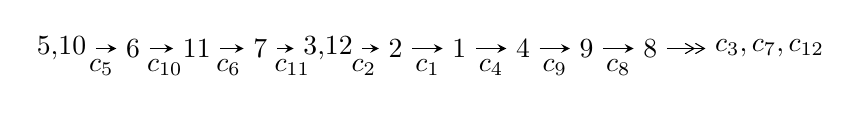
\begin{tikzpicture}[x=23pt, y=7pt]
	% node
	\node (A0) at (-1/8, 0) {5,10};
	\node (A1) at (1, 0) {6};
	\node (A2) at (2, 0) {11};
	\node (A3) at (3, 0) {7};
	\node (A4) at (65/16, 0) {3,12};
	\node (A5) at (41/8, 0) {2};
	\node (A6) at (49/8, 0) {1};
	\node (A7) at (57/8, 0) {4};
	\node (A8) at (65/8, 0) {9};
	\node (A9) at (73/8, 0) {8};
	\node (C1) at (1/2, -1) {$c_{5}$};
	\node (C2) at (3/2, -1) {$c_{10}$};
	\node (C3) at (5/2, -1) {$c_{6}$};
	\node (C4) at (7/2, -1) {$c_{11}$};
	\node (C5) at (37/8, -1) {$c_{2}$};
	\node (C6) at (45/8, -1) {$c_{1}$};
	\node (C7) at (53/8, -1) {$c_{4}$};
	\node (C8) at (61/8, -1) {$c_{9}$};
	\node (C9) at (69/8, -1) {$c_{8}$};
	\node (A10) at (11, 0) {$c_{3},c_{7},c_{12}$};

	% edge
	\draw[->,>=stealth]	
	(A0) edge (A1) (A1) edge (A2) (A2) edge (A3) (A3) edge (A4) (A4) edge (A5) (A5) edge (A6) (A6) edge (A7) (A7) edge (A8) (A8) edge (A9) ;
	\draw[->>,>={angle 60}]	
	(A9) edge (A10);
\end{tikzpicture} \\ 

\end{tabular} \\

\footnotetext{
The image of knot diagram is generated by the software ``\textbf{Draw programme}" developed by Andrew Bartholomew(\url{http://www.layer8.co.uk/maths/draw/index.htm\#Running-draw}), where we modified some parts for our purpose(\url{https://github.com/CATsTAILs/LinksPainter}).
}\phantom \\ \newline 
\centering \textbf{Ideals for irreducible components\footnotemark of $X_{\text{par}}$} 
 
\begin{align*}
I^u_{1}&=\langle 
u^{29}- u^{28}+\cdots+b+1,\;- u^{29}+u^{28}+\cdots+a+6 u,\;u^{30}-2 u^{29}+\cdots-36 u^3-1\rangle \\
I^u_{2}&=\langle 
b+1,\;a,\;u^3+u^2-2 u-1\rangle \\
\\
\end{align*}
\raggedright * 2 irreducible components of $\dim_{\mathbb{C}}=0$, with total 33 representations.\\
\footnotetext{All coefficients of polynomials are rational numbers. But the coefficients are sometimes approximated in decimal forms when there is not enough margin.}
\newpage
\renewcommand{\arraystretch}{1}
\centering \section*{I. $I^u_{1}= \langle u^{29}- u^{28}+\cdots+b+1,\;- u^{29}+u^{28}+\cdots+a+6 u,\;u^{30}-2 u^{29}+\cdots-36 u^3-1 \rangle$}
\flushleft \textbf{(i) Arc colorings}\\
\begin{tabular}{m{7pt} m{180pt} m{7pt} m{180pt} }
\flushright $a_{5}=$&$\begin{pmatrix}1\\0\end{pmatrix}$ \\
\flushright $a_{10}=$&$\begin{pmatrix}0\\u\end{pmatrix}$ \\
\flushright $a_{6}=$&$\begin{pmatrix}1\\- u^2\end{pmatrix}$ \\
\flushright $a_{11}=$&$\begin{pmatrix}u\\- u^3+u\end{pmatrix}$ \\
\flushright $a_{7}=$&$\begin{pmatrix}- u^2+1\\u^4-2 u^2\end{pmatrix}$ \\
\flushright $a_{3}=$&$\begin{pmatrix}u^{29}- u^{28}+\cdots-8 u^2-6 u\\- u^{29}+u^{28}+\cdots-2 u-1\end{pmatrix}$ \\
\flushright $a_{12}=$&$\begin{pmatrix}- u^3+2 u\\u^5-3 u^3+u\end{pmatrix}$ \\
\flushright $a_{2}=$&$\begin{pmatrix}- u^{14}+11 u^{12}+\cdots-8 u-1\\- u^{29}+u^{28}+\cdots-2 u-1\end{pmatrix}$ \\
\flushright $a_{1}=$&$\begin{pmatrix}- u^5+4 u^3-3 u\\u^7-5 u^5+6 u^3- u\end{pmatrix}$ \\
\flushright $a_{4}=$&$\begin{pmatrix}- u^{29}+u^{28}+\cdots-6 u-1\\- u^{29}+u^{28}+\cdots- u-1\end{pmatrix}$ \\
\flushright $a_{9}=$&$\begin{pmatrix}- u^6+5 u^4-6 u^2+1\\u^8-6 u^6+10 u^4-4 u^2\end{pmatrix}$ \\
\flushright $a_{8}=$&$\begin{pmatrix}u^4-3 u^2+1\\- u^6+4 u^4-3 u^2\end{pmatrix}$\\&\end{tabular}
\flushleft \textbf{(ii) Obstruction class $= -1$}\\~\\
\flushleft \textbf{(iii) Cusp Shapes $= -3 u^{29}+4 u^{28}+62 u^{27}-82 u^{26}-561 u^{25}+739 u^{24}+2918 u^{23}-3849 u^{22}-9630 u^{21}+12801 u^{20}+21006 u^{19}-28320 u^{18}-30675 u^{17}+42061 u^{16}+30044 u^{15}-41342 u^{14}-20264 u^{13}+26026 u^{12}+10788 u^{11}-10222 u^{10}-5598 u^9+2750 u^8+2538 u^7-619 u^6-778 u^5+21 u^4+168 u^3+52 u^2-25 u+7$}\\~\\
\newpage\renewcommand{\arraystretch}{1}
\flushleft \textbf{(iv) u-Polynomials at the component}\newline \\
\begin{tabular}{m{50pt}|m{274pt}}
Crossings & \hspace{64pt}u-Polynomials at each crossing \\
\hline $$\begin{aligned}c_{1}\end{aligned}$$&$\begin{aligned}
&u^{30}+12 u^{29}+\cdots+97 u+1
\end{aligned}$\\
\hline $$\begin{aligned}c_{2},c_{4}\end{aligned}$$&$\begin{aligned}
&u^{30}-4 u^{29}+\cdots+13 u-1
\end{aligned}$\\
\hline $$\begin{aligned}c_{3},c_{9}\end{aligned}$$&$\begin{aligned}
&u^{30}- u^{29}+\cdots-28 u+8
\end{aligned}$\\
\hline $$\begin{aligned}c_{5},c_{6},c_{7}\\c_{8},c_{10},c_{11}\\c_{12}\end{aligned}$$&$\begin{aligned}
&u^{30}+2 u^{29}+\cdots+36 u^3-1
\end{aligned}$\\
\hline
\end{tabular}\\~\\
\newpage\renewcommand{\arraystretch}{1}
\flushleft \textbf{(v) Riley Polynomials at the component}\newline \\
\begin{tabular}{m{50pt}|m{274pt}}
Crossings & \hspace{64pt}Riley Polynomials at each crossing \\
\hline $$\begin{aligned}c_{1}\end{aligned}$$&$\begin{aligned}
&y^{30}+16 y^{29}+\cdots-7313 y+1
\end{aligned}$\\
\hline $$\begin{aligned}c_{2},c_{4}\end{aligned}$$&$\begin{aligned}
&y^{30}-12 y^{29}+\cdots-97 y+1
\end{aligned}$\\
\hline $$\begin{aligned}c_{3},c_{9}\end{aligned}$$&$\begin{aligned}
&y^{30}-21 y^{29}+\cdots-1104 y+64
\end{aligned}$\\
\hline $$\begin{aligned}c_{5},c_{6},c_{7}\\c_{8},c_{10},c_{11}\\c_{12}\end{aligned}$$&$\begin{aligned}
&y^{30}-46 y^{29}+\cdots+40 y^2+1
\end{aligned}$\\
\hline
\end{tabular}\\~\\
\newpage\flushleft \textbf{(vi) Complex Volumes and Cusp Shapes}
$$\begin{array}{c|c|c}  
\text{Solutions to }I^u_{1}& \I (\text{vol} + \sqrt{-1}CS) & \text{Cusp shape}\\
 \hline 
\begin{aligned}
u &= \phantom{-}0.900406 + 0.238240 I \\
a &= -0.659304 - 0.413832 I \\
b &= \phantom{-}0.605232 + 0.768254 I\end{aligned}
 & \phantom{-}5.67065 + 1.25696 I & \phantom{-}15.5737 - 1.7388 I \\ \hline\begin{aligned}
u &= \phantom{-}0.900406 - 0.238240 I \\
a &= -0.659304 + 0.413832 I \\
b &= \phantom{-}0.605232 - 0.768254 I\end{aligned}
 & \phantom{-}5.67065 - 1.25696 I & \phantom{-}15.5737 + 1.7388 I \\ \hline\begin{aligned}
u &= \phantom{-}0.814325 + 0.340165 I \\
a &= \phantom{-}0.69999 + 1.77618 I \\
b &= \phantom{-}1.030380 - 0.688639 I\end{aligned}
 & \phantom{-}4.42916 + 6.78890 I & \phantom{-}12.9792 - 7.4265 I \\ \hline\begin{aligned}
u &= \phantom{-}0.814325 - 0.340165 I \\
a &= \phantom{-}0.69999 - 1.77618 I \\
b &= \phantom{-}1.030380 + 0.688639 I\end{aligned}
 & \phantom{-}4.42916 - 6.78890 I & \phantom{-}12.9792 + 7.4265 I \\ \hline\begin{aligned}
u &= \phantom{-}1.18737\phantom{ +0.000000I} \\
a &= \phantom{-}0.321529\phantom{ +0.000000I} \\
b &= \phantom{-}0.549343\phantom{ +0.000000I}\end{aligned}
 & \phantom{-}5.59474\phantom{ +0.000000I} & \phantom{-}18.0870\phantom{ +0.000000I} \\ \hline\begin{aligned}
u &= -0.736617 + 0.129687 I \\
a &= \phantom{-}0.52614 + 2.05833 I \\
b &= -0.816371 - 0.432342 I\end{aligned}
 & \phantom{-}0.97252 - 1.81198 I & \phantom{-}11.73549 + 4.66948 I \\ \hline\begin{aligned}
u &= -0.736617 - 0.129687 I \\
a &= \phantom{-}0.52614 - 2.05833 I \\
b &= -0.816371 + 0.432342 I\end{aligned}
 & \phantom{-}0.97252 + 1.81198 I & \phantom{-}11.73549 - 4.66948 I \\ \hline\begin{aligned}
u &= \phantom{-}0.654424\phantom{ +0.000000I} \\
a &= -0.551259\phantom{ +0.000000I} \\
b &= -1.18483\phantom{ +0.000000I}\end{aligned}
 & -0.312115\phantom{ +0.000000I} & \phantom{-}16.4990\phantom{ +0.000000I} \\ \hline\begin{aligned}
u &= -1.37237\phantom{ +0.000000I} \\
a &= \phantom{-}0.0265788\phantom{ +0.000000I} \\
b &= -1.33306\phantom{ +0.000000I}\end{aligned}
 & \phantom{-}6.56541\phantom{ +0.000000I} & \phantom{-}13.9410\phantom{ +0.000000I} \\ \hline\begin{aligned}
u &= \phantom{-}1.393080 + 0.049142 I \\
a &= \phantom{-}0.62086 - 1.75059 I \\
b &= -0.838747 + 0.622252 I\end{aligned}
 & \phantom{-}8.15659 + 2.43505 I & \phantom{-}13.02410 - 2.90794 I\\
 \hline 
 \end{array}$$\newpage$$\begin{array}{c|c|c}  
\text{Solutions to }I^u_{1}& \I (\text{vol} + \sqrt{-1}CS) & \text{Cusp shape}\\
 \hline 
\begin{aligned}
u &= \phantom{-}1.393080 - 0.049142 I \\
a &= \phantom{-}0.62086 + 1.75059 I \\
b &= -0.838747 - 0.622252 I\end{aligned}
 & \phantom{-}8.15659 - 2.43505 I & \phantom{-}13.02410 + 2.90794 I \\ \hline\begin{aligned}
u &= -1.41889 + 0.15784 I \\
a &= \phantom{-}0.01368 - 1.73786 I \\
b &= \phantom{-}1.114240 + 0.728134 I\end{aligned}
 & \phantom{-}11.8944 - 8.6308 I & \phantom{-}14.0718 + 5.7224 I \\ \hline\begin{aligned}
u &= -1.41889 - 0.15784 I \\
a &= \phantom{-}0.01368 + 1.73786 I \\
b &= \phantom{-}1.114240 - 0.728134 I\end{aligned}
 & \phantom{-}11.8944 + 8.6308 I & \phantom{-}14.0718 - 5.7224 I \\ \hline\begin{aligned}
u &= -0.348859 + 0.441668 I \\
a &= \phantom{-}0.229073 - 0.720707 I \\
b &= \phantom{-}0.785869 - 0.632862 I\end{aligned}
 & \phantom{-}1.73384 + 0.97008 I & \phantom{-}10.55280 + 0.95390 I \\ \hline\begin{aligned}
u &= -0.348859 - 0.441668 I \\
a &= \phantom{-}0.229073 + 0.720707 I \\
b &= \phantom{-}0.785869 + 0.632862 I\end{aligned}
 & \phantom{-}1.73384 - 0.97008 I & \phantom{-}10.55280 - 0.95390 I \\ \hline\begin{aligned}
u &= -1.45263 + 0.10165 I \\
a &= -0.661962 + 1.037750 I \\
b &= \phantom{-}0.546899 - 0.940788 I\end{aligned}
 & \phantom{-}13.61630 - 2.52281 I & \phantom{-}16.2553 + 0. I\phantom{ +0.000000I} \\ \hline\begin{aligned}
u &= -1.45263 - 0.10165 I \\
a &= -0.661962 - 1.037750 I \\
b &= \phantom{-}0.546899 + 0.940788 I\end{aligned}
 & \phantom{-}13.61630 + 2.52281 I & \phantom{-}16.2553 + 0. I\phantom{ +0.000000I} \\ \hline\begin{aligned}
u &= -0.206383 + 0.495565 I \\
a &= \phantom{-}1.71927 - 0.54217 I \\
b &= \phantom{-}0.926515 + 0.641729 I\end{aligned}
 & \phantom{-}1.28497 - 4.02644 I & \phantom{-}8.41488 + 6.42284 I \\ \hline\begin{aligned}
u &= -0.206383 - 0.495565 I \\
a &= \phantom{-}1.71927 + 0.54217 I \\
b &= \phantom{-}0.926515 - 0.641729 I\end{aligned}
 & \phantom{-}1.28497 + 4.02644 I & \phantom{-}8.41488 - 6.42284 I \\ \hline\begin{aligned}
u &= -0.362782\phantom{ +0.000000I} \\
a &= \phantom{-}0.804898\phantom{ +0.000000I} \\
b &= \phantom{-}0.108164\phantom{ +0.000000I}\end{aligned}
 & \phantom{-}0.561369\phantom{ +0.000000I} & \phantom{-}17.6530\phantom{ +0.000000I}\\
 \hline 
 \end{array}$$\newpage$$\begin{array}{c|c|c}  
\text{Solutions to }I^u_{1}& \I (\text{vol} + \sqrt{-1}CS) & \text{Cusp shape}\\
 \hline 
\begin{aligned}
u &= \phantom{-}0.118463 + 0.232287 I \\
a &= -1.31174 - 2.44567 I \\
b &= -0.912796 + 0.166074 I\end{aligned}
 & -1.60535 + 0.58110 I & -1.83750 - 2.62782 I \\ \hline\begin{aligned}
u &= \phantom{-}0.118463 - 0.232287 I \\
a &= -1.31174 + 2.44567 I \\
b &= -0.912796 - 0.166074 I\end{aligned}
 & -1.60535 - 0.58110 I & -1.83750 + 2.62782 I \\ \hline\begin{aligned}
u &= -1.79109\phantom{ +0.000000I} \\
a &= \phantom{-}0.214755\phantom{ +0.000000I} \\
b &= \phantom{-}0.718711\phantom{ +0.000000I}\end{aligned}
 & \phantom{-}16.5830\phantom{ +0.000000I} & \phantom{-0.000000 } 0 \\ \hline\begin{aligned}
u &= \phantom{-}1.83755\phantom{ +0.000000I} \\
a &= \phantom{-}0.242340\phantom{ +0.000000I} \\
b &= -1.40717\phantom{ +0.000000I}\end{aligned}
 & \phantom{-}18.6422\phantom{ +0.000000I} & \phantom{-0.000000 } 0 \\ \hline\begin{aligned}
u &= -1.84184 + 0.01166 I \\
a &= \phantom{-}0.64542 + 1.69046 I \\
b &= -0.867094 - 0.716132 I\end{aligned}
 & -19.1326 - 2.7360 I & \phantom{-0.000000 } 0 \\ \hline\begin{aligned}
u &= -1.84184 - 0.01166 I \\
a &= \phantom{-}0.64542 - 1.69046 I \\
b &= -0.867094 + 0.716132 I\end{aligned}
 & -19.1326 + 2.7360 I & \phantom{-0.000000 } 0 \\ \hline\begin{aligned}
u &= \phantom{-}1.84728 + 0.04017 I \\
a &= -0.22651 + 1.65159 I \\
b &= \phantom{-}1.166510 - 0.750722 I\end{aligned}
 & -15.2987 + 9.6434 I & \phantom{-0.000000 } 0 \\ \hline\begin{aligned}
u &= \phantom{-}1.84728 - 0.04017 I \\
a &= -0.22651 - 1.65159 I \\
b &= \phantom{-}1.166510 + 0.750722 I\end{aligned}
 & -15.2987 - 9.6434 I & \phantom{-0.000000 } 0 \\ \hline\begin{aligned}
u &= \phantom{-}1.85511 + 0.02516 I \\
a &= -0.624328 - 1.260080 I \\
b &= \phantom{-}0.533783 + 1.034720 I\end{aligned}
 & -13.33250 + 3.18487 I & \phantom{-0.000000 } 0 \\ \hline\begin{aligned}
u &= \phantom{-}1.85511 - 0.02516 I \\
a &= -0.624328 + 1.260080 I \\
b &= \phantom{-}0.533783 - 1.034720 I\end{aligned}
 & -13.33250 - 3.18487 I & \phantom{-0.000000 } 0\\
 \hline 
 \end{array}$$\newpage\newpage\renewcommand{\arraystretch}{1}
\centering \section*{II. $I^u_{2}= \langle b+1,\;a,\;u^3+u^2-2 u-1 \rangle$}
\flushleft \textbf{(i) Arc colorings}\\
\begin{tabular}{m{7pt} m{180pt} m{7pt} m{180pt} }
\flushright $a_{5}=$&$\begin{pmatrix}1\\0\end{pmatrix}$ \\
\flushright $a_{10}=$&$\begin{pmatrix}0\\u\end{pmatrix}$ \\
\flushright $a_{6}=$&$\begin{pmatrix}1\\- u^2\end{pmatrix}$ \\
\flushright $a_{11}=$&$\begin{pmatrix}u\\u^2- u-1\end{pmatrix}$ \\
\flushright $a_{7}=$&$\begin{pmatrix}- u^2+1\\u^2- u-1\end{pmatrix}$ \\
\flushright $a_{3}=$&$\begin{pmatrix}0\\-1\end{pmatrix}$ \\
\flushright $a_{12}=$&$\begin{pmatrix}u^2-1\\- u^2\end{pmatrix}$ \\
\flushright $a_{2}=$&$\begin{pmatrix}-1\\-1\end{pmatrix}$ \\
\flushright $a_{1}=$&$\begin{pmatrix}-1\\0\end{pmatrix}$ \\
\flushright $a_{4}=$&$\begin{pmatrix}0\\-1\end{pmatrix}$ \\
\flushright $a_{9}=$&$\begin{pmatrix}0\\u\end{pmatrix}$ \\
\flushright $a_{8}=$&$\begin{pmatrix}- u\\u\end{pmatrix}$\\&\end{tabular}
\flushleft \textbf{(ii) Obstruction class $= 1$}\\~\\
\flushleft \textbf{(iii) Cusp Shapes $= u^2+u+5$}\\~\\
\newpage\renewcommand{\arraystretch}{1}
\flushleft \textbf{(iv) u-Polynomials at the component}\newline \\
\begin{tabular}{m{50pt}|m{274pt}}
Crossings & \hspace{64pt}u-Polynomials at each crossing \\
\hline $$\begin{aligned}c_{1},c_{2}\end{aligned}$$&$\begin{aligned}
&(u-1)^3
\end{aligned}$\\
\hline $$\begin{aligned}c_{3},c_{9}\end{aligned}$$&$\begin{aligned}
&u^3
\end{aligned}$\\
\hline $$\begin{aligned}c_{4}\end{aligned}$$&$\begin{aligned}
&(u+1)^3
\end{aligned}$\\
\hline $$\begin{aligned}c_{5},c_{6},c_{7}\\c_{8}\end{aligned}$$&$\begin{aligned}
&u^3+u^2-2 u-1
\end{aligned}$\\
\hline $$\begin{aligned}c_{10},c_{11},c_{12}\end{aligned}$$&$\begin{aligned}
&u^3- u^2-2 u+1
\end{aligned}$\\
\hline
\end{tabular}\\~\\
\newpage\renewcommand{\arraystretch}{1}
\flushleft \textbf{(v) Riley Polynomials at the component}\newline \\
\begin{tabular}{m{50pt}|m{274pt}}
Crossings & \hspace{64pt}Riley Polynomials at each crossing \\
\hline $$\begin{aligned}c_{1},c_{2},c_{4}\end{aligned}$$&$\begin{aligned}
&(y-1)^3
\end{aligned}$\\
\hline $$\begin{aligned}c_{3},c_{9}\end{aligned}$$&$\begin{aligned}
&y^3
\end{aligned}$\\
\hline $$\begin{aligned}c_{5},c_{6},c_{7}\\c_{8},c_{10},c_{11}\\c_{12}\end{aligned}$$&$\begin{aligned}
&y^3-5 y^2+6 y-1
\end{aligned}$\\
\hline
\end{tabular}\\~\\
\newpage\flushleft \textbf{(vi) Complex Volumes and Cusp Shapes}
$$\begin{array}{c|c|c}  
\text{Solutions to }I^u_{2}& \I (\text{vol} + \sqrt{-1}CS) & \text{Cusp shape}\\
 \hline 
\begin{aligned}
u &= \phantom{-}1.24698\phantom{ +0.000000I} \\
a &= \phantom{-0.000000 } 0 \\
b &= -1.00000\phantom{ +0.000000I}\end{aligned}
 & \phantom{-}4.69981\phantom{ +0.000000I} & \phantom{-}7.80190\phantom{ +0.000000I} \\ \hline\begin{aligned}
u &= -0.445042\phantom{ +0.000000I} \\
a &= \phantom{-0.000000 } 0 \\
b &= -1.00000\phantom{ +0.000000I}\end{aligned}
 & -0.939962\phantom{ +0.000000I} & \phantom{-}4.75300\phantom{ +0.000000I} \\ \hline\begin{aligned}
u &= -1.80194\phantom{ +0.000000I} \\
a &= \phantom{-0.000000 } 0 \\
b &= -1.00000\phantom{ +0.000000I}\end{aligned}
 & \phantom{-}15.9794\phantom{ +0.000000I} & \phantom{-}6.44500\phantom{ +0.000000I}\\
 \hline 
 \end{array}$$\newpage
\newpage\renewcommand{\arraystretch}{1}
\centering \section*{ III. u-Polynomials}
\begin{tabular}{m{50pt}|m{274pt}}
Crossings & \hspace{64pt}u-Polynomials at each crossing \\
\hline $$\begin{aligned}c_{1}\end{aligned}$$&$\begin{aligned}
&((u-1)^3)(u^{30}+12 u^{29}+\cdots+97 u+1)
\end{aligned}$\\
\hline $$\begin{aligned}c_{2}\end{aligned}$$&$\begin{aligned}
&((u-1)^3)(u^{30}-4 u^{29}+\cdots+13 u-1)
\end{aligned}$\\
\hline $$\begin{aligned}c_{3},c_{9}\end{aligned}$$&$\begin{aligned}
&u^3(u^{30}- u^{29}+\cdots-28 u+8)
\end{aligned}$\\
\hline $$\begin{aligned}c_{4}\end{aligned}$$&$\begin{aligned}
&((u+1)^3)(u^{30}-4 u^{29}+\cdots+13 u-1)
\end{aligned}$\\
\hline $$\begin{aligned}c_{5},c_{6},c_{7}\\c_{8}\end{aligned}$$&$\begin{aligned}
&(u^3+u^2-2 u-1)(u^{30}+2 u^{29}+\cdots+36 u^3-1)
\end{aligned}$\\
\hline $$\begin{aligned}c_{10},c_{11},c_{12}\end{aligned}$$&$\begin{aligned}
&(u^3- u^2-2 u+1)(u^{30}+2 u^{29}+\cdots+36 u^3-1)
\end{aligned}$\\
\hline
\end{tabular}\newpage\renewcommand{\arraystretch}{1}
\centering \section*{ IV. Riley Polynomials}
\begin{tabular}{m{50pt}|m{274pt}}
Crossings & \hspace{64pt}Riley Polynomials at each crossing \\
\hline $$\begin{aligned}c_{1}\end{aligned}$$&$\begin{aligned}
&((y-1)^3)(y^{30}+16 y^{29}+\cdots-7313 y+1)
\end{aligned}$\\
\hline $$\begin{aligned}c_{2},c_{4}\end{aligned}$$&$\begin{aligned}
&((y-1)^3)(y^{30}-12 y^{29}+\cdots-97 y+1)
\end{aligned}$\\
\hline $$\begin{aligned}c_{3},c_{9}\end{aligned}$$&$\begin{aligned}
&y^3(y^{30}-21 y^{29}+\cdots-1104 y+64)
\end{aligned}$\\
\hline $$\begin{aligned}c_{5},c_{6},c_{7}\\c_{8},c_{10},c_{11}\\c_{12}\end{aligned}$$&$\begin{aligned}
&(y^3-5 y^2+6 y-1)(y^{30}-46 y^{29}+\cdots+40 y^2+1)
\end{aligned}$\\
\hline
\end{tabular}
\vskip 2pc
\end{document}